% !TEX root = ../main.tex

\chapter{Object Reconstruction}

The ATLAS detector records signals produced by particles traversing its tracking
systems, calorimeters, and muon spectrometer.
Before these detector-level measurements can be used in physics analyses, they
must be translated into a coherent description of each event.
This translation is achieved through reconstruction algorithms that combine raw
detector information with calibration procedures to define high-level physics
objects.

Object reconstruction provides the interface between the detector and the
analysis.
Reconstructed objects—such as tracks, vertices, leptons, jets, and missing
transverse momentum—are designed to approximate the kinematic properties of the
underlying particles while remaining robust against detector effects and
pile-up.
Their definitions therefore reflect analysis-driven trade-offs between
efficiency, resolution, background rejection, and systematic uncertainties.

This chapter describes the reconstruction of the physics objects relevant for the
analyses presented in this thesis.
The discussion focuses primarily on the Run~2 ATLAS reconstruction framework,
which forms the basis of the results presented here, and concludes with a brief
overview of key developments introduced in Run~3.

\section{Tracks and Vertices}

Charged-particle trajectories reconstructed in the ID provide the most precise
measurements of the momenta and production vertices of particles produced in
$pp$ collisions.
Tracking information constitutes a core ingredient for vertex reconstruction,
lepton identification, flavour tagging, pile-up mitigation, and the reconstruction
of global event observables.
Track reconstruction proceeds through a sequence of well-defined steps:
detector measurements are clustered into space points, which are used to seed
track candidates that are subsequently extended, fitted, and disambiguated.
The resulting tracks form the basis of primary-vertex reconstruction, while
displaced tracks are further exploited to identify secondary vertices.
Muon reconstruction follows the same general principles and is discussed
separately in Section~\ref{sec:reco-muons}~\cite{ATLASTrackingDense2017}.

Track reconstruction in the ID starts from the formation of clusters in the pixel
and SCT detectors.
Adjacent readout channels with signals above threshold are aggregated into
clusters, which constitute the basic hit objects for pattern recognition.
These clusters are converted into three-dimensional measurement points (space
points) with associated uncertainties.
For pixel detectors, a single cluster typically yields a space point directly,
whereas for the SCT the three-dimensional position is obtained by combining
the stereo information from the two sides of a strip module.

Track seeds are formed by combining reconstructed space points, providing an
initial estimate of the track parameters under the assumption of a helical
trajectory in the magnetic field.
Track finding follows an iterative combinatorial strategy, in which track
candidates are extended layer by layer by incorporating compatible space points
using a combinatorial Kalman filter.
If multiple compatible extensions exist on a given detector layer, several
track candidates are propagated in parallel, increasing the reconstruction
efficiency in dense environments~\cite{Fruhwirth1987KalmanTrackVertex}.

The large number of track candidates produced by the combinatorial procedure
necessitates an ambiguity-resolution stage.
Track candidates are ranked according to a quality score that reflects the number
and quality of associated measurements, the goodness of the track fit, and the
track kinematics.
Candidates are processed in descending order of this score, and conflicts arising
from shared measurements are resolved by retaining the most probable track
hypotheses.
In dense environments, multiple charged particles may contribute to a single
detector cluster.
To mitigate the resulting loss in reconstruction efficiency, dedicated
neural-network-based algorithms are employed to identify merged clusters and to
guide the ambiguity-resolution procedure~\cite{ATLASPixelNNClustering2014}.
For track candidates surviving ambiguity resolution, a high-resolution fit is
performed using all associated measurements.
The resulting fitted tracks constitute the final ID track collection.

The primary vertex (PV) is identified as the vertex with the largest summed track
activity, commonly quantified by the $\sum p_T^2$ of its associated tracks.
Accurate PV reconstruction is essential for pile-up suppression and for
associating reconstructed objects with the hard-scatter interaction.
PV reconstruction typically consists of three steps:
(i) associating reconstructed tracks to common points of origin,
(ii) fitting the vertex position using track parameters and their covariances,
and (iii) selecting the vertex corresponding to the hard-scatter interaction in
the presence of pile-up.
The PV position and its resolution depend on the event track multiplicity and
track-parameter uncertainties; at high pile-up, additional effects such as vertex
merging and track mis-assignment can degrade both reconstruction and selection
performance~\cite{ATLASPrimaryVertices2017}.

An important ingredient in vertex reconstruction is the measurement of the
luminous region (beam spot) and its evolution in time.
Knowledge of the beam spot can be used as an external constraint in the vertex
fit, improving the transverse vertex-position resolution and stabilising the
reconstruction performance as pile-up increases.
The PV reconstruction performance has been studied in Run~2 data, and practical
parameterisations are provided to model the reconstruction efficiency and the
impact of vertex merging at high pile-up~\cite{ATLASPrimaryVertices2017}.

Secondary vertices (SVs) are reconstructed by identifying groups of displaced
tracks inconsistent with originating from the PV and fitting them to a common
point of origin.
Such vertices arise from decays of long-lived hadrons, in particular heavy-flavour
hadrons, as well as from other displaced topologies such as photon conversions and
$V^0$ decays.
The SV position, its displacement from the PV (often expressed through a decay-
length significance), the track multiplicity, and fit-quality observables provide
powerful inputs to flavour tagging and other lifetime-based measurements.

\section{Electrons and Photons}

Electrons and photons are reconstructed by combining information from the inner
tracking detector and the electromagnetic calorimeter.
During Run~2, ATLAS transitioned from a fixed-size sliding-window clustering
approach to a reconstruction strategy based on topological cell clusters and
variable-size superclusters.
This evolution improves the energy containment for electrons affected by
bremsstrahlung in the tracking material and for photons undergoing conversion
before reaching the calorimeter~\cite{ATLASeGammaPerformance2019,ATLASegammaTopoSuperclusters2017}.
This section summarises the reconstruction and selection ingredients most relevant
for physics analyses.

\subsection{Topo-clusters}

The reconstruction of electrons and photons is based on topological clusters
(topo-clusters) built from calorimeter cells.
Topo-clusters are seeded and grown according to the signal significance of
individual calorimeter cells,
\begin{equation}
\varsigma^{\mathrm{EM}}_{\mathrm{cell}} \equiv
\frac{E^{\mathrm{EM}}_{\mathrm{cell}}}{\sigma^{\mathrm{EM}}_{\mathrm{noise,cell}}},
\end{equation}
where $E^{\mathrm{EM}}_{\mathrm{cell}}$ is the reconstructed cell energy at the
electromagnetic calibration scale and $\sigma^{\mathrm{EM}}_{\mathrm{noise,cell}}$
denotes the expected cell noise, including both electronics noise and an estimate
of the pile-up contribution.
In the standard ``4--2--0'' configuration, proto-clusters are seeded by cells with
$|\varsigma^{\mathrm{EM}}_{\mathrm{cell}}|\ge 4$, grown by iteratively adding
neighbouring cells with $|\varsigma^{\mathrm{EM}}_{\mathrm{cell}}|\ge 2$, and
finally augmented by a crown of adjacent cells.
To suppress noise-induced clusters, cells in the presampler and the first
electromagnetic layer are excluded from the seeding stage.
Proto-clusters containing multiple local maxima can be split into separate
clusters.

For electron and photon reconstruction, only the electromagnetic energy of
topo-clusters is considered, with a dedicated treatment of the barrel--endcap
transition region.
A preselection on the electromagnetic energy fraction is applied to suppress
pile-up-induced clusters, yielding a collection of EM topo-clusters that serve as
inputs to subsequent track matching and supercluster construction.
Topo-clusters thus provide noise-suppressed, three-dimensional calorimeter energy
building blocks, while higher-level clustering is required to recover the full
energy of individual electromagnetic objects~\cite{ATLASeGammaPerformance2019,
ATLASegammaTopoSuperclusters2017}.

\subsection{Tracks and Conversions}

Electron reconstruction relies critically on tracking information.
Electron tracks may undergo substantial energy loss through bremsstrahlung in the
material of the tracking detector, leading to biases in the fitted track
parameters and degraded track--cluster matching.
To mitigate these effects, tracks associated with electromagnetic regions of
interest are refitted using bremsstrahlung-aware algorithms, most notably a
Gaussian-sum-filter (GSF) refit, which provides an improved estimate of the track
parameters in the presence of radiative energy loss~\cite{ATLASGSF2012}.
The characteristic impact of bremsstrahlung on the track trajectory and the
associated calorimeter energy deposits is illustrated in
Fig.~\ref{fig:reco-egamma-electron-track}.

\begin{figure}
	\centering
  	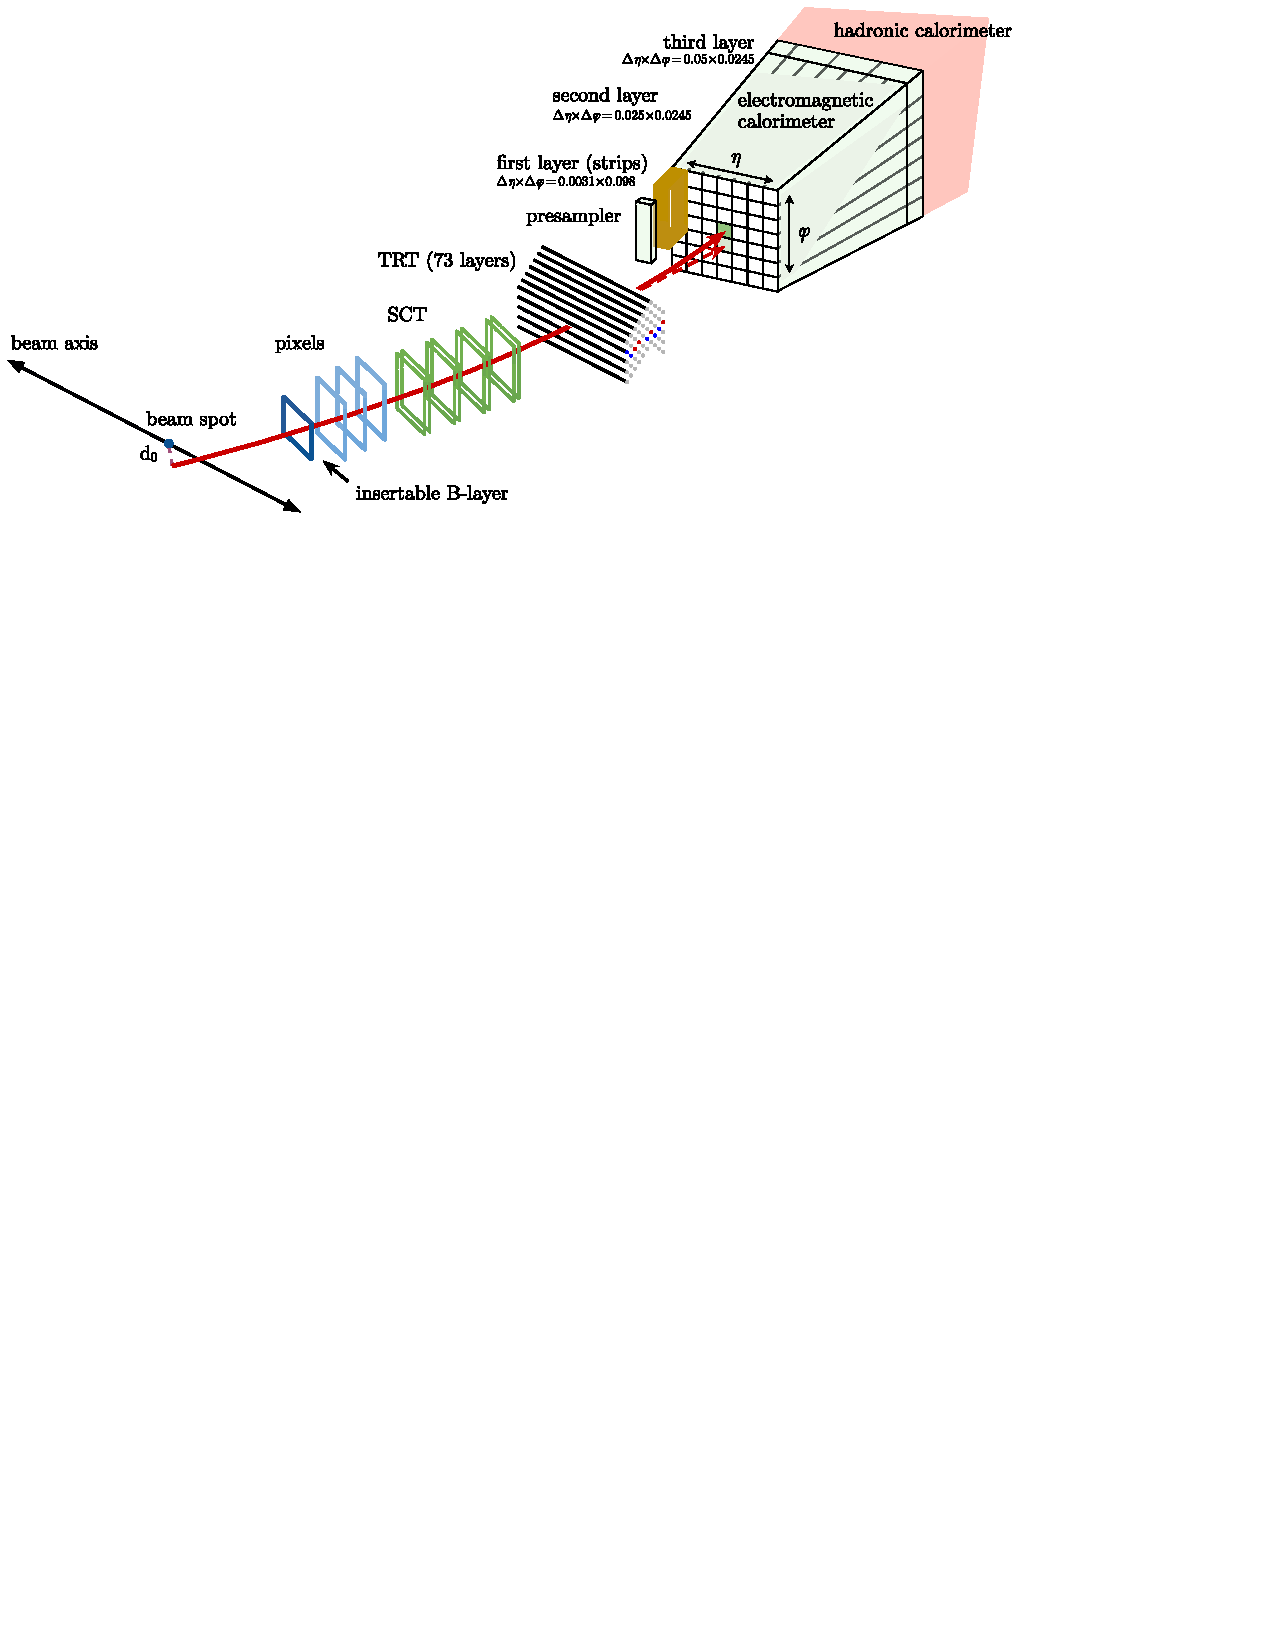
\includegraphics[width=0.9\textwidth]{figures/Track_of_electron.pdf}
	\caption{Illustration of bremsstrahlung effects on electron tracks and
	calorimeter energy deposits. Taken from Ref.~\cite{ATLASeGammaPerformance2019}.}
	\label{fig:reco-egamma-electron-track}
\end{figure}

Tracks are matched to EM topo-clusters by extrapolating them to the second
electromagnetic calorimeter layer and requiring compatibility in $(\eta,\phi)$.
For electrons with significant energy loss, the track momentum can be rescaled to
the cluster energy for the purpose of extrapolation, improving the matching
efficiency.

Photons may convert into an $e^+e^-$ pair in the detector material upstream of the
calorimeter.
Such photon conversions are reconstructed by identifying conversion vertices
formed from pairs of oppositely charged tracks, and in specific topologies from
single-track conversions.
The reconstructed conversion vertices are matched to EM topo-clusters and later
to photon superclusters.
They are used both to classify photons as converted or unconverted and to improve
the purity and energy reconstruction of the photon sample~\cite{ATLASeGammaPerformance2019}.

\subsection{Superclusters}

In the presence of bremsstrahlung (for electrons) or conversions (for photons),
the electromagnetic energy associated with a single particle can be distributed
across multiple spatially separated calorimeter deposits.
As a result, a single fixed-size cluster may fail to capture the full energy of
the object.
This motivates a variable-size clustering strategy in which multiple related EM
topo-clusters are aggregated into a single supercluster.

Superclusters are constructed by first identifying a seed EM topo-cluster and
then iteratively adding nearby satellite clusters consistent with bremsstrahlung
photons, conversion-related topologies, or cluster splitting.
This dynamic clustering approach improves energy containment and provides a more
robust calorimeter reference for subsequent track and conversion-vertex matching.
The superclustering concept is illustrated in
Fig.~\ref{fig:reco-egamma-superclustering}~\cite{ATLASegammaTopoSuperclusters2017}.

\begin{figure}
	\centering
  	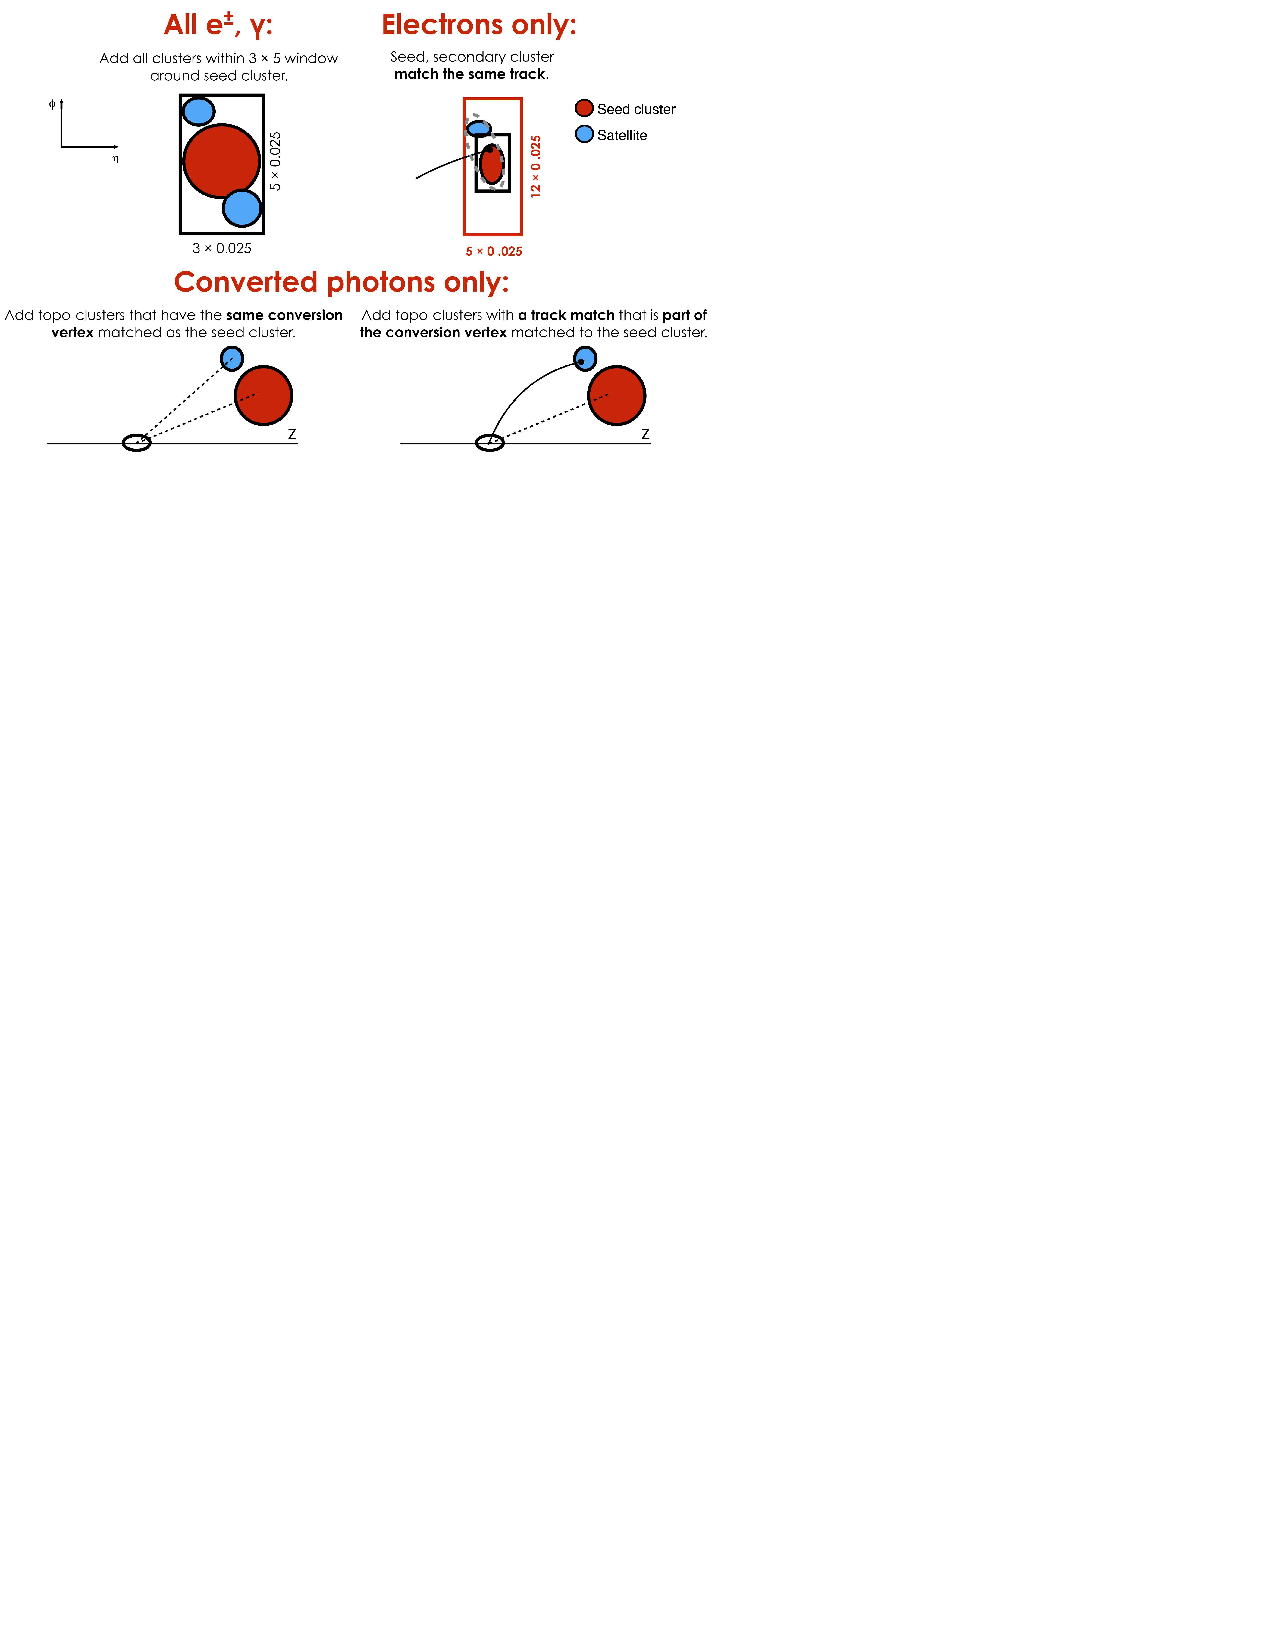
\includegraphics[width=0.9\textwidth]{figures/superclustering.pdf}
	\caption{Illustration of the superclustering procedure for electrons and
	photons. Taken from Ref.~\cite{ATLASegammaTopoSuperclusters2017}.}
	\label{fig:reco-egamma-superclustering}
\end{figure}

After supercluster construction, tracks are matched to electron superclusters,
while conversion vertices are matched to photon superclusters.
Analysis-level objects are defined accordingly: electrons correspond to a
supercluster with a matched track, converted photons to a supercluster with a
matched conversion vertex, and unconverted photons to a supercluster without such
matches.
Since the electron and photon reconstruction chains proceed independently, a
given calorimeter seed may give rise to both an electron and a photon candidate.
An ambiguity-resolution procedure is therefore applied to suppress clear
misclassifications while retaining a controlled overlap for borderline cases,
which can be handled at the analysis level~\cite{ATLASeGammaPerformance2019}.

\subsection{Identification}

After reconstruction, identification selections are applied to enhance the
purity of prompt isolated electrons and photons.
ATLAS employs a likelihood-based discriminant constructed from variables measured
in the tracking detector, the electromagnetic calorimeter, and their combination.
The discriminating power arises from the characteristic electromagnetic shower
shapes in the calorimeter, the compatibility between the calorimeter cluster and
an associated track (for electrons), and track-quality and impact-parameter
information.

In this thesis, a detailed discussion of the full set of low-level input
variables is not required.
Representative examples include the hadronic leakage variable
$R_{\mathrm{had}}$, shower-shape observables in the strip and middle layers (such
as $R_{\eta}$ and $w_{\eta 2}$), track--cluster matching variables
($\Delta\eta_1$, $\Delta\phi_{\mathrm{res}}$), and, for tighter electron
selections, consistency observables such as the ratio of calorimeter energy to
track momentum, $E/p$.

For electrons, likelihood operating points—commonly referred to as Loose, Medium,
and Tight—are defined through requirements on the discriminant and are
complemented by additional criteria to suppress specific backgrounds, in
particular converted photons and non-prompt electrons.
Typical additions for tighter selections include stricter requirements on the
track momentum and on the consistency between the track momentum and the
reconstructed cluster energy, as well as conversion-related vetoes.

The corresponding identification efficiencies are measured in data using
tag-and-probe techniques in $Z\to ee$ events and are typically presented as
functions of the electron transverse energy and pseudorapidity.
Representative results for the standard operating points are shown in
Fig.~\ref{fig:reco-egamma-electron-id-eff}~\cite{ATLASeGammaPerformance2019,
ATLASElectronRecoID2019}.

\begin{figure}[tb]
  \centering
  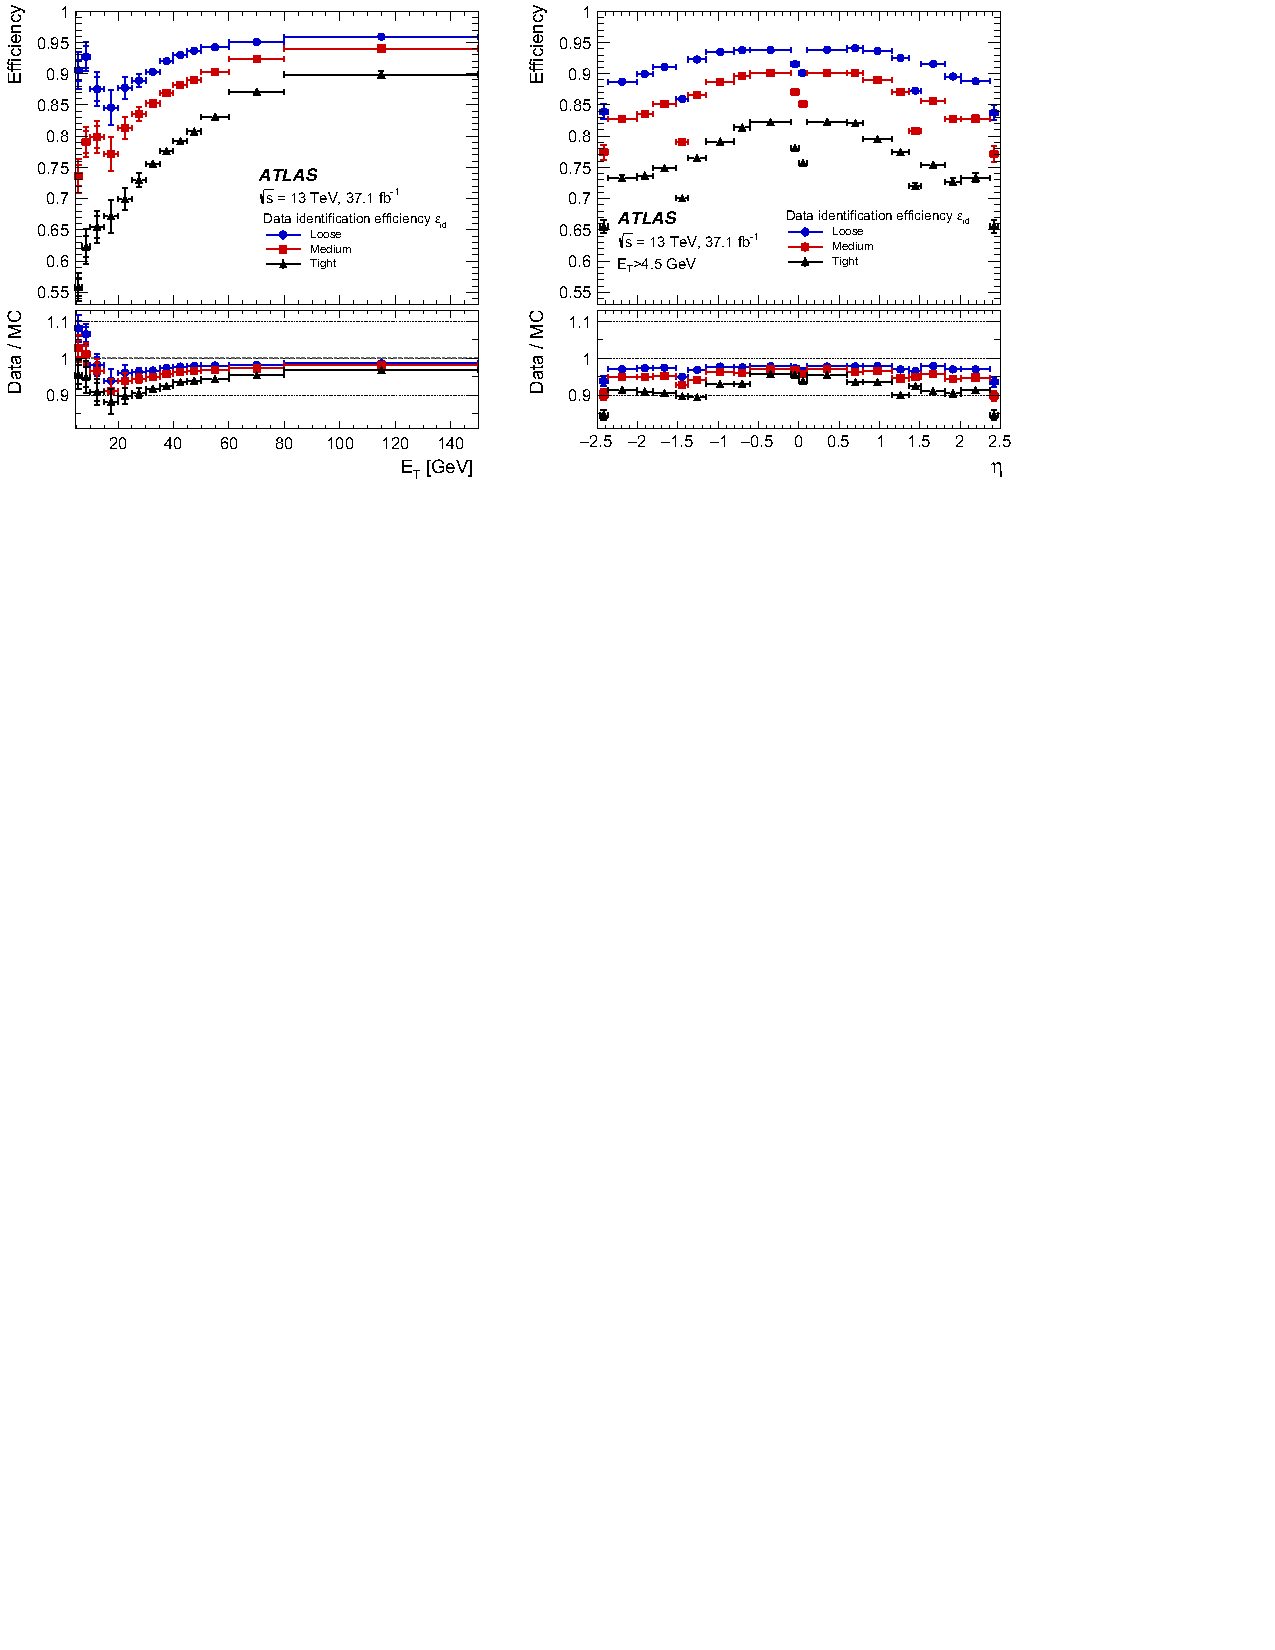
\includegraphics[width=0.88\textwidth]{figures/Electron_id_eff.pdf}
  \caption{
    Measured likelihood-based electron identification efficiencies in
    $Z\to ee$ events for the Loose, Medium, and Tight operating points as
    functions of $E_T$ and $\eta$.
    Taken from Ref.~\cite{ATLASElectronRecoID2019}.
  }
  \label{fig:reco-egamma-electron-id-eff}
\end{figure}

\subsection{Isolation}

Isolation requirements are applied to suppress non-prompt electrons, such as those
originating from heavy-flavour decays, and jets misidentified as electrons, while
maintaining high efficiency for prompt isolated leptons.
Isolation can be defined using calorimeter energy deposits and/or nearby tracks.

Calorimeter-based isolation is constructed from the transverse energy of
topo-clusters in a cone around the electron or photon direction, with the core
energy of the electromagnetic object subtracted and additional corrections
applied to account for residual leakage and pile-up contributions.
Track-based isolation is computed from the scalar sum of track transverse momenta
within a cone around the lepton direction, excluding tracks matched to the lepton
itself and requiring compatibility with the PV.
For electrons, variable-size cones are commonly used to preserve efficiency for
boosted topologies.

Standard isolation working points are defined in Run~2 to balance background
rejection against signal efficiency, and are calibrated using data-driven
techniques.
These working points are used in this thesis following the standard ATLAS
recommendations~\cite{ATLASeGammaPerformance2019,ATLASElectronRecoID2019}.

\section{Muons}
\label{sec:reco-muons}

Muon reconstruction in ATLAS combines tracking information from the ID and the
Muon Spectrometer (MS), complemented by calorimeter information primarily used
to model the energy loss of muons traversing the calorimeter systems.
This multi-detector approach provides redundancy and enables robust muon
reconstruction over a wide range of pseudorapidity and transverse momentum.
During Run~2, the reconstruction and identification algorithms were re-optimised
to maintain high efficiency and purity under high pile-up conditions while
preserving good momentum resolution in both the low- and high-$p_T$ regimes%
~\cite{ATLASMuonReco2021,ATLASMuonReco2016}.

\subsection{Reconstruction}

Muon reconstruction proceeds in stages, starting from track reconstruction in the
MS and followed by the combination of MS and ID information to form analysis-level
muon candidates.
In the MS, reconstruction begins with the identification of local track segments
in individual muon stations.
In the bending plane, segments are constructed from precision chamber hits,
primarily from Monitored Drift Tubes (MDTs) and Cathode Strip Chambers (CSCs) in
the forward region, by searching for aligned hit patterns and fitting them with
straight lines.
Pattern recognition at this stage can be formulated using voting-based techniques,
such as a Hough transform, to identify consistent track hypotheses.

To build three-dimensional track candidates, the segment information in the
bending plane is combined with the measurement of the non-bending coordinate
provided by the trigger chambers (RPCs in the barrel and TGCs in the endcaps).
Segments reconstructed in different MS stations are then linked into preliminary
track candidates using a loose pointing constraint towards the interaction
region and an approximate description of the bending in the toroidal magnetic
field.

Candidate trajectories are subsequently refined with a global $\chi^2$ fit
through the full magnetic-field map.
The fit incorporates material effects and can account for residual alignment
uncertainties between chambers, which is essential to maintain a controlled
momentum resolution at high $p_T$.
After the initial fit, outlier hits may be removed and additional compatible hits
along the trajectory can be recovered, after which the fit is repeated.
Finally, the fitted MS track parameters are corrected for the expected energy loss
in the calorimeters and extrapolated back to the interaction point, providing the
stand-alone MS track parameters used in later combination and identification
steps~\cite{ATLASMuonReco2021}.

For analysis-level muons, ATLAS combines ID and MS information using several
complementary reconstruction strategies.
The availability of multiple muon types mitigates acceptance gaps and
reconstruction failure modes, and enables analyses to trade efficiency against
purity and momentum resolution depending on the kinematic regime of interest.
The main reconstructed muon types are:

\begin{itemize}
  \item \textbf{Combined (CB)} muons are formed by matching an MS track to an ID
  track and performing a combined refit using the full set of ID and MS
  measurements, together with calorimeter energy-loss modelling.
  This is the nominal muon type for most analyses, providing high purity and good
  momentum resolution over a broad $p_T$ range.

  \item \textbf{Inside-out combined (IO)} muons start from an ID track extrapolated
  to the MS, where compatible MS hits are associated and used in a combined
  refit.
  This strategy recovers efficiency when an independent MS track is not
  reconstructed, for example for low-$p_T$ muons that do not cross all MS stations
  or in regions with reduced MS coverage.

  \item \textbf{MS-extrapolated (ME)} muons correspond to MS tracks that cannot be
  matched to an ID track and are extrapolated back to the beam line.
  This category extends the muon acceptance beyond the ID tracking coverage and
  is particularly relevant in the forward region.

  \item \textbf{Segment-tagged (ST)} muons are ID tracks that are tagged as muons
  by matching to at least one reconstructed MS segment with tight angular
  compatibility.
  The muon kinematics are typically taken from the ID track fit, while the MS
  segment provides an identification handle.

  \item \textbf{Calorimeter-tagged (CT)} muons are ID tracks identified as muons
  using calorimeter energy deposits consistent with a minimum-ionising particle
  along the extrapolated track.
  As for ST muons, the kinematics are taken from the ID track fit, while the tag
  provides MS-independent muon identification.
\end{itemize}

Dedicated reconstruction variants are employed to improve performance near the
boundaries of the ID acceptance.
For example, silicon-associated forward (SiF) muons exploit short silicon track
segments to enhance matching and refit performance for forward muons where full
ID tracking information is not available~\cite{ATLASMuonReco2021}.

\subsection{Identification}

After reconstruction, muon candidates are selected using identification working
points (WPs).
Each WP corresponds to a defined set of requirements on the underlying ID track
quality, such as hit content and fit quality, on the availability and quality of
MS information, and on compatibility observables between the ID and MS
measurements when both are present.
These requirements suppress backgrounds from hadrons misidentified as muons,
such as decays in flight or punch-through, and reject poorly reconstructed tracks
that would otherwise degrade the momentum resolution.

ATLAS provides a hierarchy of standard identification WPs, commonly named Loose,
Medium and Tight, which offer increasing purity at the cost of decreasing
efficiency.
The Medium WP is typically used as a baseline in physics analyses, while the Loose
WP can recover efficiency in challenging reconstruction regimes, in particular at
low $p_T$.
The Tight WP increases background rejection and improves the robustness of the
momentum measurement by applying stricter quality and compatibility requirements.
In addition, dedicated WPs target extreme regions of phase space.
The High-$p_T$ WP focuses on optimising the momentum resolution and rejecting
muons with large measurement uncertainties or problematic MS configurations,
while the Low-$p_T$ WP is designed to preserve efficiency for muons of only a few
GeV; both cut-based and multivariate variants are provided~\cite{ATLASMuonReco2021}.

Representative reconstruction and identification efficiencies for the standard
working points are measured in data using tag-and-probe techniques in
$Z\to\mu\mu$ and $J/\psi\to\mu\mu$ events and compared to simulation, as shown in
Fig.~\ref{fig:reco-muon-wp-eff}.

\begin{figure}
	\centering
  	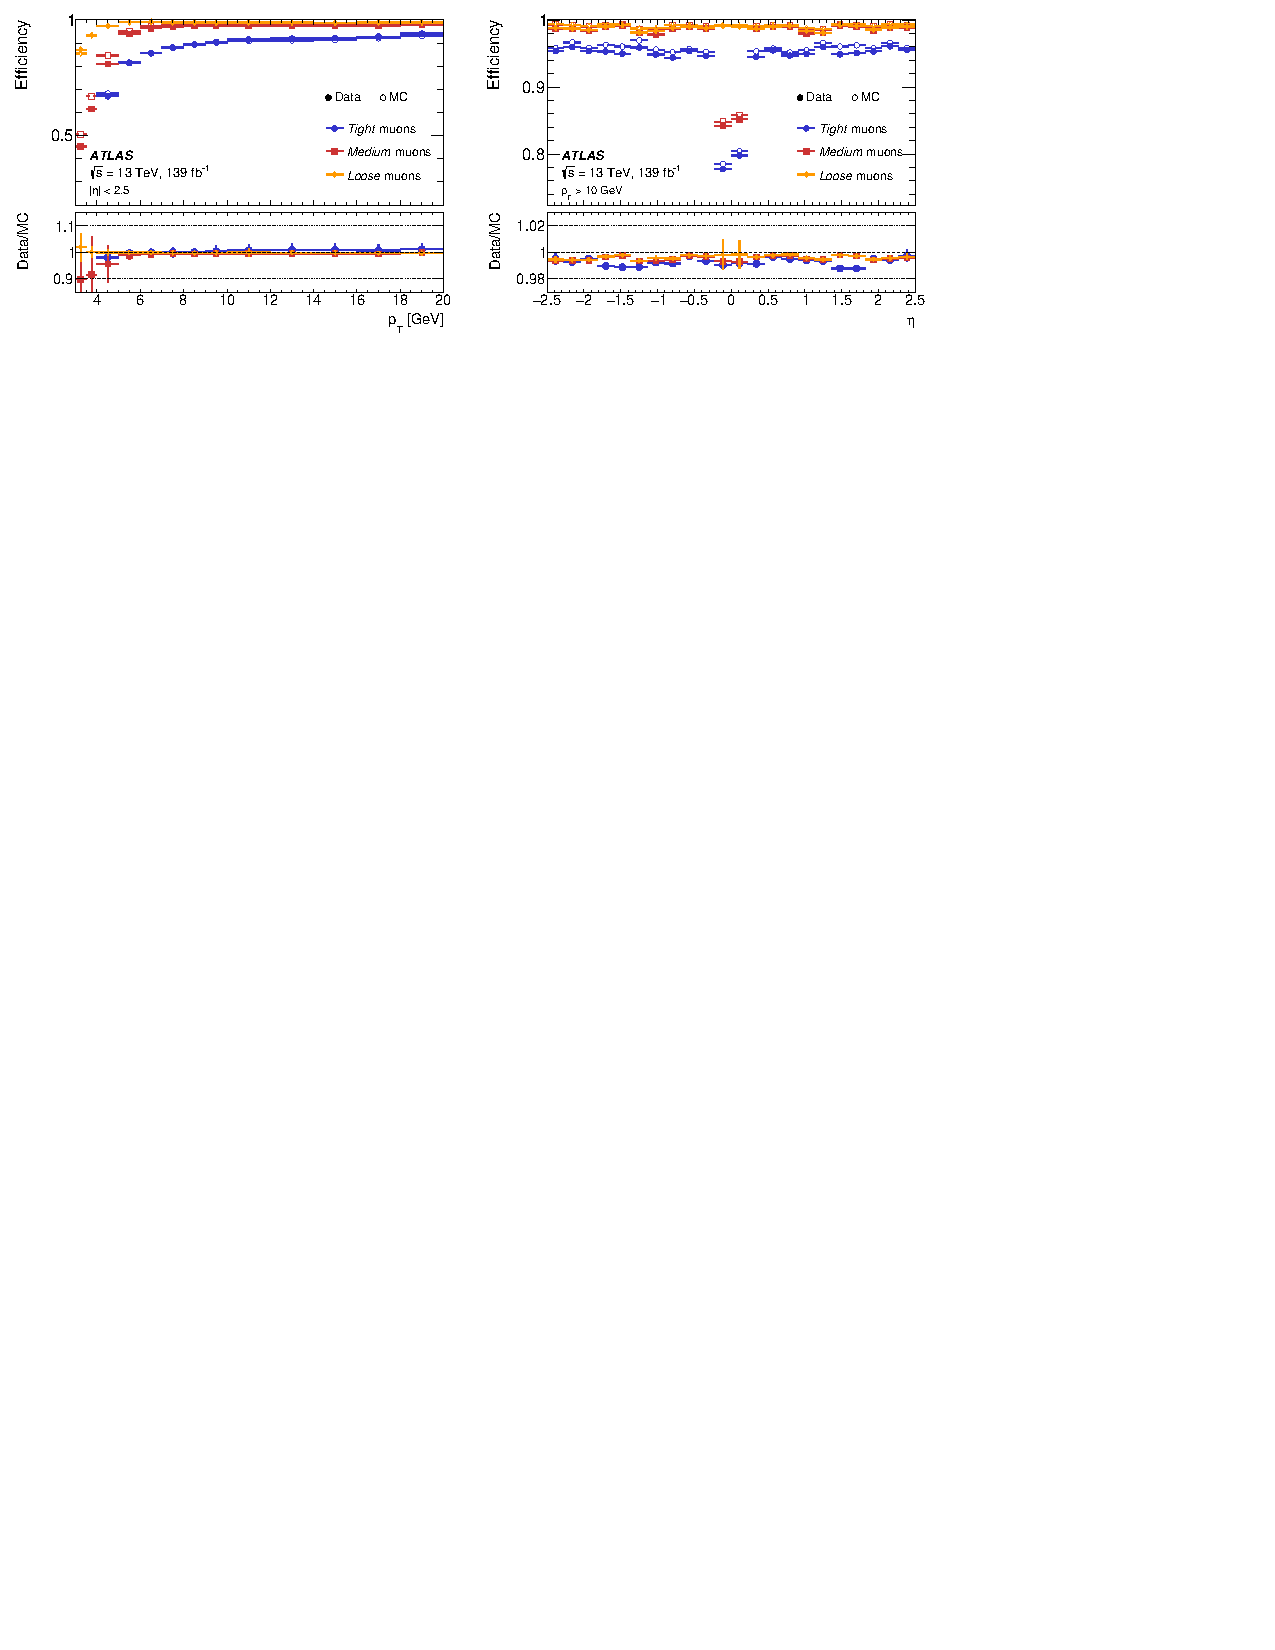
\includegraphics[width=0.9\textwidth]{figures/Muon_WP_Eff.pdf}
	\caption{Muon reconstruction and identification efficiencies for standard
	working points as a function of muon $p_T$ and $\eta$. Taken from
	Ref.~\cite{ATLASMuonReco2021}.}
	\label{fig:reco-muon-wp-eff}
\end{figure}

\subsection{Vertex Association and Isolation}

To select prompt muons originating from the hard-scatter interaction, vertex
association requirements are applied, typically based on transverse and
longitudinal impact parameters with respect to the PV.
These requirements reduce contamination from secondary muons produced in
heavy-flavour decays or in-flight decays of hadrons.

Isolation criteria provide additional discrimination against non-prompt and
non-isolated muons.
Isolation can be defined using nearby tracks and/or calorimeter activity within a
cone around the muon direction.
Pile-up sensitivity is reduced by selecting tracks compatible with the PV and by
using variable-size isolation cones that preserve efficiency for boosted
topologies.
For precision measurements, the efficiencies of vertex association and isolation
selections are determined with data-driven techniques, most prominently
tag-and-probe methods in $Z\to\mu\mu$ and $J/\psi\to\mu\mu$ decays.
The resulting data-to-simulation ratios are provided as scale factors that are
applied in analyses to correct simulated samples and propagate the associated
systematic uncertainties~\cite{ATLASMuonReco2021}.

\section{Flavour Tagging}

Flavour tagging refers to the identification of jets originating from heavy-flavour
quarks, in particular $b$- and $c$-quarks.
In this thesis, flavour tagging enters the analysis exclusively through the
per-jet output discriminant provided by the DL1r algorithm.
The purpose of this section is therefore to describe, from an analysis-oriented
perspective, how the DL1r discriminant is constructed from reconstructed objects,
how it relates to earlier Run~2 flavour-tagging algorithms, and how it is used
and calibrated in physics analyses.

\subsection{From Run~2 taggers to DL1r}

ATLAS flavour tagging in Run~2 follows a paradigm in which lifetime-sensitive
information is extracted from reconstructed objects and combined into a single
high-level discriminant.
Early Run~2 algorithms relied on explicit feature engineering and boosted-decision-
tree-based classifiers, most notably the MV2 series.
In parallel, dedicated vertexing algorithms such as JetFitter were developed to
exploit the characteristic topology of heavy-flavour decay chains.
These approaches provided strong performance, but were limited in their ability
to capture complex correlations among the input observables.

More recent developments adopt deep-learning-based strategies that provide a more
flexible and powerful combination of the available information.
The DL1 family of algorithms represents the baseline deep-learning flavour-tagging
approach in Run~2 ATLAS, and DL1r is the specific configuration used in this
analysis.
The evolution of flavour-tagging performance during Run~2 is illustrated in
Fig.~\ref{fig:btag_performance_comparison}, which compares representative Run~2
taggers and highlights the significant improvement in light-jet rejection
achieved by deep-learning-based approaches at a fixed $b$-jet efficiency.

\begin{figure}[t]
  \centering
  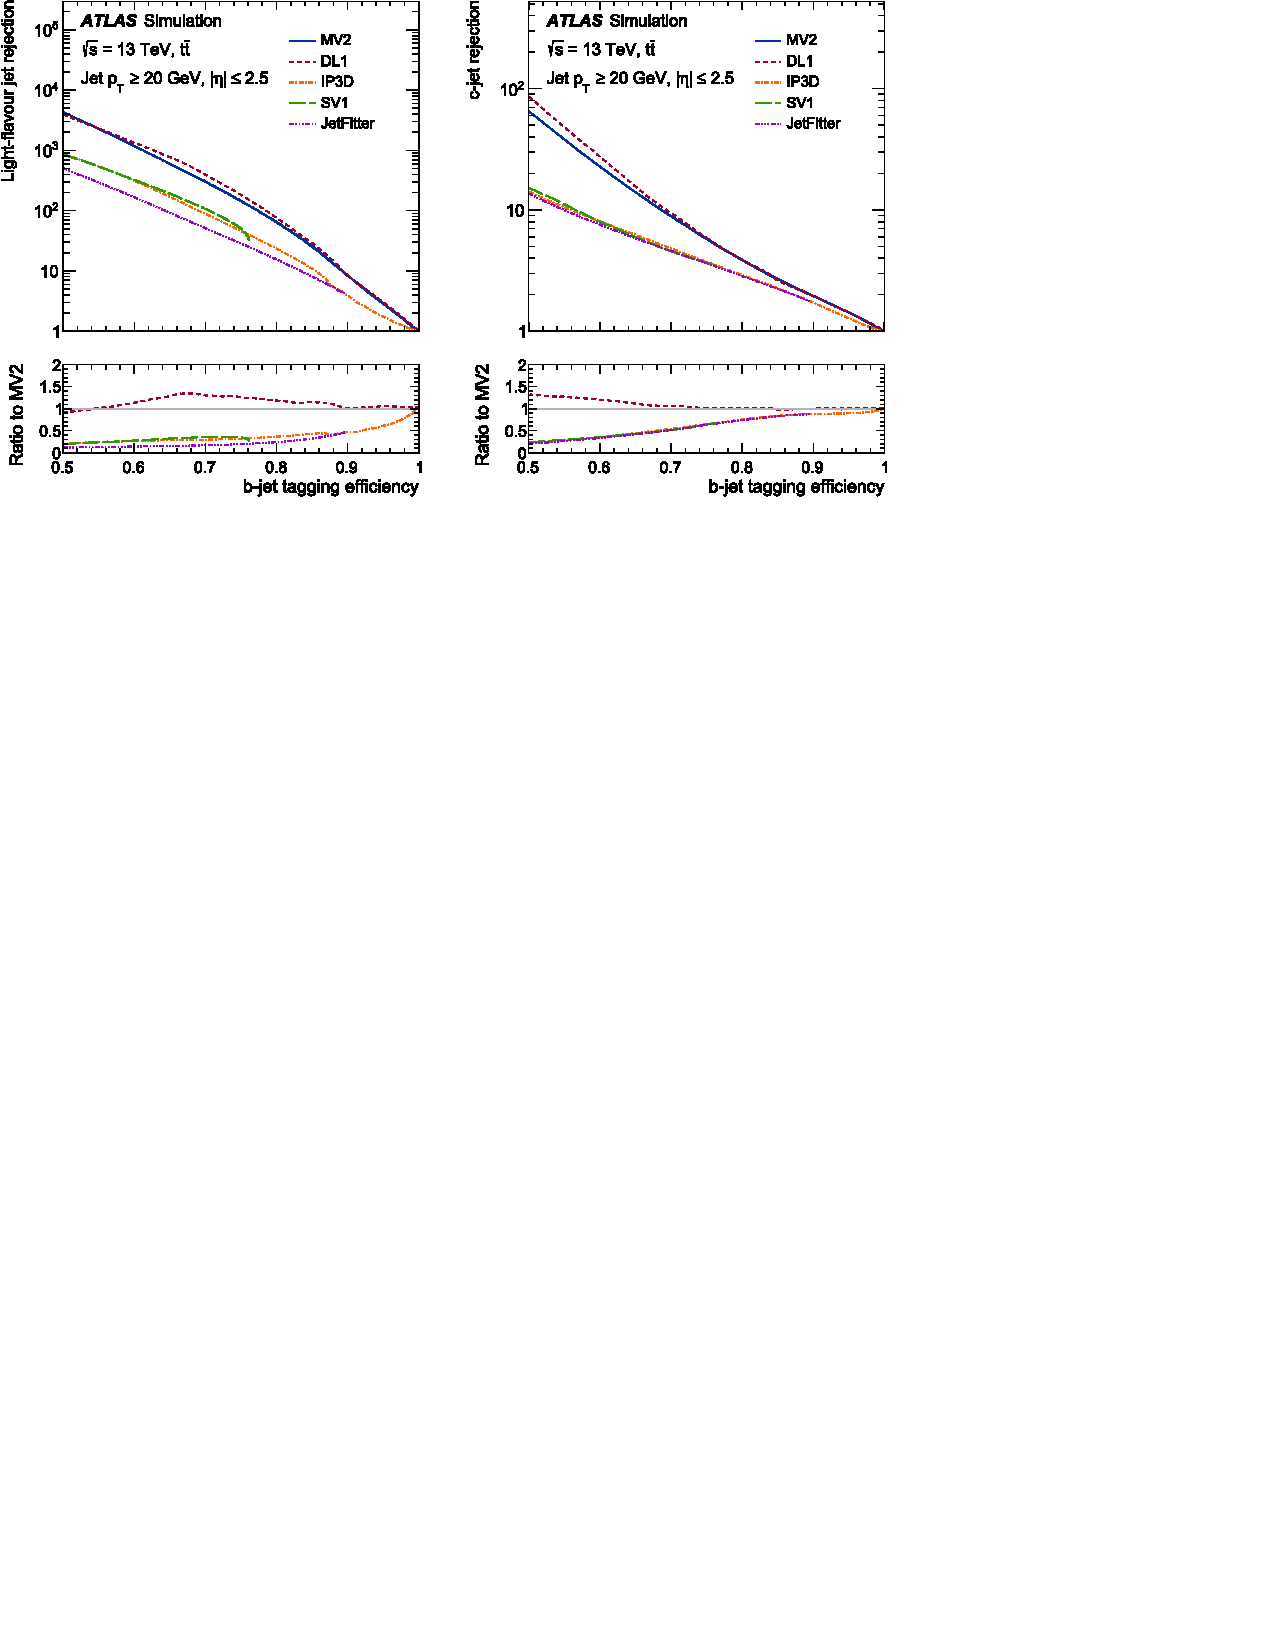
\includegraphics[width=0.9\textwidth]{figures/b-tagging_eff.pdf}
  \caption{
    Comparison of $b$-tagging performance for representative Run~2 ATLAS
    flavour-tagging algorithms.
    The light-jet (left) and $c$-jet (right) rejection is shown as a function of
    the $b$-jet efficiency for simulated $t\bar{t}$ events at $\sqrt{s}=13$~TeV.
    Taken from Ref.~\cite{ATLASFlavourTaggingRun2Dataset2023}.
  }
  \label{fig:btag_performance_comparison}
\end{figure}

\subsection{DL1r discriminant}

The DL1r algorithm combines information from the reconstructed jet, tracks
associated with the jet, and reconstructed secondary vertices into a multi-class
neural network.
The network outputs per-jet probabilities $p_b$, $p_c$, and
$p_{\mathrm{light}}$ for the jet to originate from a $b$-quark, a $c$-quark, or a
light-flavour parton, respectively.

Lifetime-sensitive input observables include track impact-parameter information
with respect to the primary vertex and properties of reconstructed secondary
vertices.
In addition, topological vertexing algorithms such as JetFitter provide
complementary information by exploiting the expected heavy-flavour decay-chain
topology.
These observables form the basis for both earlier Run~2 taggers and the DL1 family.

For use in physics analyses, the DL1r output probabilities are combined into a
single scalar discriminant using a log-likelihood ratio.
For $b$-tagging, the standard DL1r discriminant is defined as
\begin{equation}
D_{\mathrm{DL1r}}^{b} =
\ln\left(
\frac{p_b}{f_c\,p_c + (1-f_c)\,p_{\mathrm{light}}}
\right),
\end{equation}
where $f_c$ represents the effective fraction of $c$-jets in the background
hypothesis.
The parameter $f_c$ can be chosen a posteriori to optimise the analysis sensitivity
by tuning the relative weight assigned to $c$-jet versus light-jet backgrounds.

The performance of the DL1r discriminant is commonly characterised in terms of the
rejection of light-flavour and $c$-jets as a function of the $b$-jet efficiency.
Representative performance curves are shown in Fig.~\ref{fig:btag_performance_comparison},
demonstrating the improved discrimination achieved by DL1r compared to earlier
Run~2 algorithms.

\subsection{Working points and calibration}

In physics analyses, flavour-tagging requirements are defined through fixed
$b$-jet efficiency working points, corresponding to thresholds on the DL1r
discriminant.
Common working points in Run~2 correspond to nominal $b$-jet efficiencies of
60\%, 70\%, 77\%, and 85\%, reflecting different trade-offs between signal
efficiency and background rejection.
The specific working points used in this thesis are defined in the analysis
chapter.

The flavour-tagging performance differs between simulation and data.
Tagging efficiencies and mis-tag rates are therefore measured in data using
dedicated control samples and applied to simulated events as multiplicative scale
factors.
The associated systematic uncertainties are propagated to the final analysis
results.

\section{Missing Transverse Momentum}

Missing transverse momentum ($\vec{E}^{\mathrm{miss}}_T$) provides sensitivity to
particles that escape direct detection, most notably neutrinos, through the
conservation of transverse momentum in the hard-scattering process.
In ATLAS, $\vec{E}^{\mathrm{miss}}_T$ is reconstructed using an object-based
approach that combines calibrated physics objects (the hard term) with a
residual soft term.
This strategy is designed to suppress pile-up contamination and to ensure a
unique assignment of detector signals, thereby avoiding double counting and
reducing non-physical tails~\cite{ATLASCONF2018023}.

\subsection{Definition}

The missing transverse momentum vector is defined through its Cartesian
components in the transverse plane as
\begin{equation}
\vec{E}^{\mathrm{miss}}_T \equiv
(E^{\mathrm{miss}}_x,\,E^{\mathrm{miss}}_y)
= \sum_k \vec{E}^{\mathrm{miss},k}_T ,
\end{equation}
where the index $k$ runs over the selected hard-object collections
(electrons, photons, muons, hadronic $\tau$ candidates, and jets) and the soft
term.
Each contribution $\vec{E}^{\mathrm{miss},k}_T$ corresponds to the negative
transverse momentum associated with object category $k$.
In practice, reconstructed objects are processed in a defined order so that
calorimeter clusters and tracks are assigned to mutually exclusive terms, which
minimises double counting at the detector-signal level.

The overall activity in the event is often characterised by the scalar sum
$\sum E_T$ of the transverse momenta of all reconstructed objects and the soft
term.
This quantity is closely related to the expected resolution of
$E^{\mathrm{miss}}_T$, since larger values of $\sum E_T$ typically correspond to
higher detector occupancy and increased sensitivity to pile-up and resolution
effects.
As a result, $\sum E_T$ is commonly used as a proxy for the event energy scale
when evaluating the performance of the $E^{\mathrm{miss}}_T$ reconstruction.

\subsection{Reconstruction and pile-up mitigation}

The reconstruction of $\vec{E}^{\mathrm{miss}}_T$ follows an object-based
philosophy.
The hard term is constructed from analysis-quality physics objects after the
application of their dedicated energy or momentum calibrations.
For jets, ATLAS supports both calorimeter-based jets reconstructed from
electromagnetic-scale topological clusters (EMTopo) and particle-flow (PFlow)
jets.
The PFlow approach combines tracking and calorimeter information, improving the
suppression of pile-up contributions and the overall $E^{\mathrm{miss}}_T$
performance.

Because multiple reconstructed objects may share detector signals, a dedicated
overlap-removal procedure is applied during the construction of the hard term.
This procedure resolves ambiguities between jets and nearby electrons, photons,
or hadronic $\tau$ candidates, and accounts for the energy loss of muons in the
calorimeter as well as for final-state-radiation effects.
As a result, detector signals are assigned consistently to a single object
category, suppressing double counting and reducing artificial
$E^{\mathrm{miss}}_T$ tails.

Additional pile-up mitigation is achieved by rejecting jets originating from
pile-up vertices.
In the central detector region, jet--vertex association discriminants are applied
to low-$p_T$ jets, while dedicated treatments are employed for forward jets,
where tracking information is limited, in order to control their impact on the
$E^{\mathrm{miss}}_T$ resolution.

The soft term collects reconstructed transverse momentum that is not attributed
to any selected hard object.
To reduce sensitivity to pile-up, Run~2 ATLAS employs a track-based soft term
(TST), constructed from inner-detector tracks associated with the primary vertex
and not matched to hard objects.
This choice largely suppresses contributions from pile-up interactions and
out-of-time activity.
An analogous definition is used for PFlow-based $E^{\mathrm{miss}}_T$, with
differences relative to the standard TST found to be small in practice.

\subsection{Performance}

The performance of the $E^{\mathrm{miss}}_T$ reconstruction is evaluated in terms
of its resolution and robustness against pile-up.
These properties have been extensively validated in Run~2 data and simulation
using control samples such as $Z\to\ell\ell$ events.
A representative example of the achieved $E^{\mathrm{miss}}_T$ resolution as a
function of pile-up, characterised by the number of reconstructed primary
vertices, is shown in Fig.~\ref{fig:met_performance}.

\begin{figure}[htbp]
  \centering
  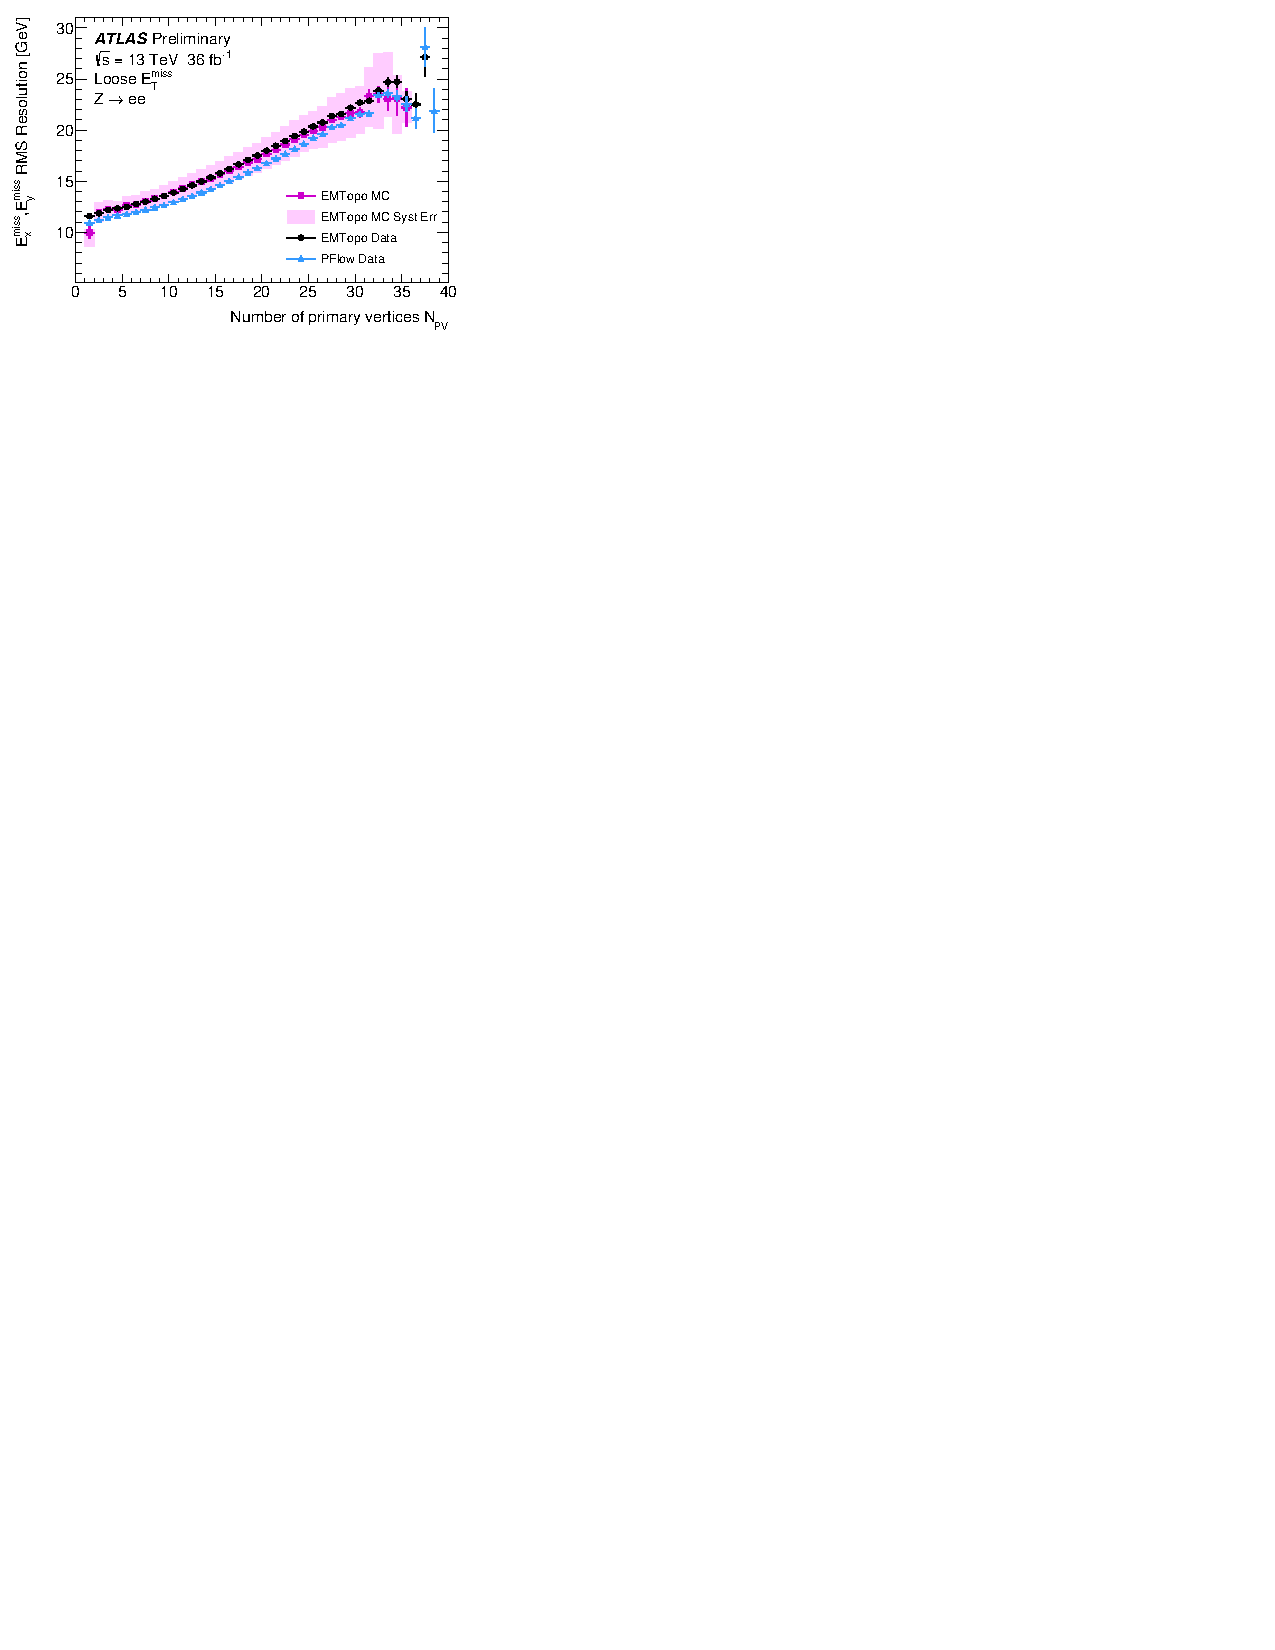
\includegraphics[width=0.6\textwidth]{figures/MET_resolution.pdf}
  \caption{
    Resolution of the $E^{\mathrm{miss}}_T$ components as a function of the number
    of reconstructed primary vertices for the baseline (Loose)
    $E^{\mathrm{miss}}_T$ reconstruction.
    Results are shown for Run~2 ATLAS data and simulation using different jet
    inputs.
    Adapted from Ref.~\cite{ATLASCONF2018023}.
  }
  \label{fig:met_performance}
\end{figure}

\section{Transition to Run~3}

The object reconstruction described in this chapter primarily reflects the
Run~2 ATLAS configuration, which forms the basis of the analyses presented in
this thesis.
The transition to Run~3 is characterised by increased instantaneous luminosity
and pile-up, together with upgrades to the detector readout and trigger systems.
These changes place stronger emphasis on reconstruction robustness, pile-up
mitigation, and the stability of physics-object definitions under more
challenging operating conditions.

In the tracking and vertexing domain, the Run~3 reconstruction framework
preserves the overall structure established in Run~2, while incorporating more
efficient pattern-recognition and track-building strategies to improve
computational performance in high pile-up environments.~\cite{ATLASTrackRecoRun3SoftwarePerf2024}
An important development is the adoption of extended large-radius ($d_0$)
tracking as a standard component, which enhances sensitivity to displaced tracks
and non-prompt signatures and is particularly relevant for searches involving
long-lived particles.~\cite{ATLASLargeImpactParameterTracks2023}
Primary-vertex reconstruction continues to rely on beam-spot constraints and
iterative vertex fitting, with refinements aimed at maintaining vertex
separation and assignment performance at higher interaction densities.

The reconstruction of electrons and photons in Run~3 retains the Run~2 object
definitions, including bremsstrahlung-aware tracking, supercluster-based
calorimeter reconstruction, and explicit treatment of photon conversions.
At the identification stage, however, increased use is made of machine-learning-
based techniques.
In particular, deep-neural-network-based electron identification~\cite{ATLASElectronDNNID2022} is gradually
introduced to complement or replace likelihood-based selections, providing
improved background rejection at fixed signal efficiency.
The energy calibration continues to rely on in-situ techniques, with updated
corrections and uncertainty treatments to ensure stability under the increased
pile-up and instantaneous luminosity conditions of Run~3.
In parallel, isolation definitions are refined to reduce their sensitivity to
pile-up, with the aim of maintaining identification efficiency and background
rejection performance comparable to that achieved in Run~2.

Muon reconstruction in Run~3 benefits from the full integration of the New Small
Wheel detector in the endcap regions, which significantly improves trigger and
reconstruction performance at high pseudorapidity.
The reconstruction algorithms are adapted to exploit the additional precision
measurements provided by the upgraded system, while the overall strategy of
combining inner-detector and muon-spectrometer information remains unchanged.
Momentum calibration and resolution studies continue to follow the Run~2 in-situ
approach, demonstrating that the established framework remains applicable in the
new detector configuration.

Jet reconstruction in Run~3 continues to employ the anti-$k_t$ algorithm as the
baseline jet definition, while the particle-flow paradigm evolves through the
introduction of Unified Flow Objects (UFOs)~\cite{ATLASUFOJetsArxiv2020}.
This development provides a more consistent treatment of charged and neutral
components and improves jet energy and mass reconstruction, particularly in
high-$p_T$ and boosted topologies.
In parallel, machine-learning-based calibration techniques, including
graph-neural-network~\cite{ATLASJetCalibTechniquesArxiv2023} and Bayesian~\cite{ATLASUncertaintyAwareCalibArxiv2024} approaches, are explored to further enhance
jet energy and mass resolution and to reduce systematic uncertainties.

Flavour tagging in Run~3 builds upon the deep-learning-based approach introduced
in Run~2 with the DL1 family.
New generations of flavour-tagging algorithms based on transformer and
graph-neural-network architectures (e.g.\ GN2~\cite{ATLASGN2Arxiv2025}) are progressively introduced, enabling a
more effective exploitation of track- and vertex-level information, especially
for high-momentum jets and complex decay topologies.
The calibration strategy for flavour tagging continues to follow the Run~2
paradigm, with efficiency and mis-tag rates measured in data and propagated to
analyses through scale factors.

Overall, the Run~3 reconstruction framework represents an evolutionary
development of the Run~2 approach.
While significant advances are made to address the more challenging Run~3
environment, the object definitions and reconstruction philosophy described in
this chapter remain directly applicable and provide the conceptual foundation
for both the Run~2 analysis presented in this thesis and ongoing Run~3 studies.